%%%%%%%%%%%%%%%%%%%% book.tex %%%%%%%%%%%%%%%%%%%%%%%%%%%%%
%
% sample root file for the chapters of your "monograph"
%
% Use this file as a template for your own input.
%
%%%%%%%%%%%%%%%% Springer-Verlag %%%%%%%%%%%%%%%%%%%%%%%%%%


% RECOMMENDED %%%%%%%%%%%%%%%%%%%%%%%%%%%%%%%%%%%%%%%%%%%%%%%%%%%
\documentclass[graybox,envcountchap,sectrefs]{./style/svmono}

% choose options for [] as required from the list
% in the Reference Guide

%\usepackage{mathptmx}
%\usepackage{helvet}
%\usepackage{courier}
%
\usepackage{type1cm}         

\usepackage{makeidx}         % allows index generation
\usepackage{graphicx}        % standard LaTeX graphics tool
                             % when including figure files
\usepackage{multicol}        % used for the two-column index
\usepackage[bottom]{footmisc}% places footnotes at page bottom

\usepackage{newtxtext}       % 
\usepackage{newtxmath}       % selects Times Roman as basic font
\usepackage{./style/code}    % custom package for listings
\usepackage{float}           % for floating figures
\usepackage{wrapfig}         % for wrapping text around figures

% see the list of further useful packages
% in the Reference Guide

\makeindex             % used for the subject index
                       % please use the style svind.ist with
                       % your makeindex program

%%%%%%%%%%%%%%%%%%%%%%%%%%%%%%%%%%%%%%%%%%%%%%%%%%%%%%%%%%%%%%%%%%%%%

\graphicspath{{./}{images/}}

\begin{document}

\author{Samuel J. Cavazos}
\title{Algebraic Geometry \& Machine Learning}
\subtitle{in Python for parseltongues}
\maketitle

\frontmatter%%%%%%%%%%%%%%%%%%%%%%%%%%%%%%%%%%%%%%%%%%%%%%%%%%%%%%


%%%%%%%%%%%%%%%%%%%%%%% dedic.tex %%%%%%%%%%%%%%%%%%%%%%%%%%%%%%%%%
%
% sample dedication
%
% Use this file as a template for your own input.
%
%%%%%%%%%%%%%%%%%%%%%%%% Springer %%%%%%%%%%%%%%%%%%%%%%%%%%

\begin{dedication}
To Adalyn \& Luka
\end{dedication}





%%%%%%%%%%%%%%%%%%%%%%%foreword.tex%%%%%%%%%%%%%%%%%%%%%%%%%%%%%%%%%
% sample foreword
%
% Use this file as a template for your own input.
%
%%%%%%%%%%%%%%%%%%%%%%%% Springer %%%%%%%%%%%%%%%%%%%%%%%%%%

\foreword

%% Please have the foreword written here
Use the template \textit{foreword.tex} together with the document class SVMono (monograph-type books) or SVMult (edited books) to style your foreword\index{foreword}. 

The foreword covers introductory remarks preceding the text of a book that are written by a \textit{person other than the author or editor} of the book. If applicable, the foreword precedes the preface which is written by the author or editor of the book.


\vspace{\baselineskip}
\begin{flushright}\noindent
Place, month year\hfill {\it Firstname  Surname}\\
\end{flushright}



%%%%%%%%%%%%%%%%%%%%%%preface.tex%%%%%%%%%%%%%%%%%%%%%%%%%%%%%%%%%%%%%%%%%
% sample preface
%
% Use this file as a template for your own input.
%
%%%%%%%%%%%%%%%%%%%%%%%% Springer %%%%%%%%%%%%%%%%%%%%%%%%%%

\preface

\textbf{Differential Geometry \& Machine Learning} explores the fascinating intersection of two powerful fields: differential geometry and machine learning. While machine learning has revolutionized industries ranging from healthcare to finance, differential geometry has long been a cornerstone of advanced mathematics, providing the tools to understand the curvature and structure of spaces. The synergy between these domains offers profound insights into the mathematical foundations of machine learning and equips practitioners with powerful techniques to build more robust and explainable models.

The motivation for this book stems from the desire to bridge the gap between theory and practice. As machine learning algorithms grow increasingly complex, understanding their underlying mechanics becomes not just an academic exercise but a necessity for developing effective, interpretable, and scalable solutions. Differential geometry provides a rigorous framework to address questions about curvature, optimization, and structure within the high-dimensional spaces where these models operate.

This book begins with the basics of machine learning, using linear regression as a gateway to understanding the fundamental principles of modeling and optimization. Through accessible explanations and hands-on examples, we build a foundation that extends naturally to more complex architectures, including neural networks. From there, we delve into the tools of differential geometry, showing how concepts such as gradients, manifolds, and geodesics inform and enhance machine learning algorithms.

Key features of this book include:
\begin{itemize}
    \item \textbf{Practical Examples}: Python-based implementations and visualizations to solidify theoretical concepts.
    \item \textbf{Mathematical Rigor}: Detailed derivations and explanations that connect machine learning practices to their geometric and mathematical underpinnings.
    \item \textbf{Interdisciplinary Approach}: Insights from both machine learning and differential geometry, fostering a holistic understanding of modern AI techniques.
\end{itemize}


This book is intended for a diverse audience:
\begin{itemize}
    \item \textbf{Mathematicians} intrigued by the applications of differential geometry in contemporary AI.
    \item \textbf{Machine Learning Engineers} seeking a deeper understanding of the mathematical principles behind their tools.
    \item \textbf{Students and Educators} looking for an accessible yet rigorous resource to explore the intersection of these fields.
\end{itemize}

As we journey through this book, we will not only develop a deeper appreciation for the beauty of differential geometry but also see how it empowers us to design better, more interpretable machine learning models. Whether you are a practitioner, researcher, or student, this book invites you to explore a rich and rewarding mathematical landscape that underpins some of the most transformative technologies of our time.

\vspace{\baselineskip}
\begin{flushright}\noindent
The Rio Grande Valley\hfill {\it Samuel J. Cavazos}\\
2025 \hfill {\it DHR Health}\\
\end{flushright}



%%%%%%%%%%%%%%%%%%%%%%acknow.tex%%%%%%%%%%%%%%%%%%%%%%%%%%%%%%%%%%%%%%%%%
% sample acknowledgement chapter
%
% Use this file as a template for your own input.
%
%%%%%%%%%%%%%%%%%%%%%%%% Springer %%%%%%%%%%%%%%%%%%%%%%%%%%

\extrachap{Acknowledgements}

This project would not have been possible without the inspiration and support of my colleagues at DHR Health, whose insights and discussions have enriched the ideas presented here. I am especially grateful to the readers and learners who engage with this material—your curiosity and passion continue to drive this work forward.

\tableofcontents

%%%%%%%%%%%%%%%%%%%%%%acronym.tex%%%%%%%%%%%%%%%%%%%%%%%%%%%%%%%%%%%%%%%%%
% sample list of acronyms
%
% Use this file as a template for your own input.
%
%%%%%%%%%%%%%%%%%%%%%%%% Springer %%%%%%%%%%%%%%%%%%%%%%%%%%

\extrachap{Acronyms}

List of abbreviations\index{acronyms, list of} and symbols\index{symbols, list of} used in the book.

\begin{description}[CABR]
\item[$\mathbb{C}$]{The field of complex numbers}
\item[$\mathbb{Q}$]{The field of rational numbers} 
\item[$\mathbb{R}$]{The field of real numbers}
\item[$\mathbb{Z}$]{The ring of integers}
\item[$\mathbb{Z}/n\mathbb{Z}$]{The ring of integers modulo $n$}
\item[ML]{Acronym for Machine-Learning}
\end{description}


\mainmatter%%%%%%%%%%%%%%%%%%%%%%%%%%%%%%%%%%%%%%%%%%%%%%%%%%%%%%%
%%%%%%%%%%%%%%%%%%%%%part.tex%%%%%%%%%%%%%%%%%%%%%%%%%%%%%%%%%%
% 
% sample part title
%
% Use this file as a template for your own input.
%
%%%%%%%%%%%%%%%%%%%%%%%% Springer %%%%%%%%%%%%%%%%%%%%%%%%%%

\begin{partbacktext}
\part{Regression Models}

\end{partbacktext}
%%%%%%%%%%%%%%%%%%%%% chapter.tex %%%%%%%%%%%%%%%%%%%%%%%%%%%%%%%%%
%
% sample chapter
%
% Use this file as a template for your own input.
%
%%%%%%%%%%%%%%%%%%%%%%%% Springer-Verlag %%%%%%%%%%%%%%%%%%%%%%%%%%
%\motto{Use the template \emph{chapter.tex} to style the various elements of your chapter content.}
\chapter{Linear Regression}
\label{intro} % Always give a unique label
% use \chaptermark{}
% to alter or adjust the chapter heading in the running head

\abstract*{
    This chapter introduces the principles of linear regression as a foundation for understanding the connection between differential geometry and machine learning. A simple linear model $M(x) = x\cdot W + b$ is constructed, and a loss function is used to quantify prediction errors. The chapter details the derivation of gradients for the loss with respect to the model parameters $W$ and $b$, providing insights into how these gradients guide the optimization process.
}

\abstract{
    This chapter introduces the principles of linear regression as a foundation for understanding the connection between differential geometry and machine learning. A simple linear model $M(x) = x \cdot W + b$ is constructed, and a loss function is used to quantify prediction errors. The chapter details the derivation of gradients for the loss with respect to the model parameters $W$ and $b$, providing insights into how these gradients guide the optimization process.
}

\section{Linear Models}
\label{sec:1}
Linear regressions are a fundamental tool in statistics and machine learning for modeling the relationship between a dependent variable $y$ and one or more independent variables $x$. The simplest form of linear regression is a univariate linear model\index{linear model, univariate}, which assumes a linear relationship between $y$ and $x$ of the form $y = x\cdot W + b$, where $W,b\in\mathbb{R}$ are real numbers. The model parameters $W$ and $b$ are learned from a dataset of input-output pairs $\{(x_i, y_i)\}_{i=1}^N$ by minimizing a loss function that quantifies the prediction errors of the model. 

A more general form of the linear model is:
$$M(x) = x\cdot W + b,$$
where:
\begin{itemize}
    \item $W$ is a \textbf{weight matrix} of shape $m \times d$,
    \item $x$ is a $d$-dimensional input vector,
    \item $b$ is an $m$-dimensional \textbf{bias vector}.
\end{itemize}

Here, the model $M(x)$ outputs an $m$-dimensional vector prediction. This flexibility allows linear regression to handle scenarios where the model predicts multiple outputs simultaneously, making it applicable to a wide range of machine learning tasks. We begin by studying the univariate case.

\section{Univariate Linear Models}
\label{sec:2}
% Always give a unique label
% and use \ref{<label>} for cross-references
% and \cite{<label>} for bibliographic references
% use \sectionmark{}
% to alter or adjust the section heading in the running head
Let's construct some data to work with that follows a somewhat linear trend and build a machine-learning model from scratch. We'll take the function $f(x)=x^2+2\cdot x+1$ over a random sample of points in $[0,10]$ and add some uniform noise.

\lstinputlisting[language=Python]{Regression/code/1.1.1.1.py}

\begin{figure}[H]
\centering
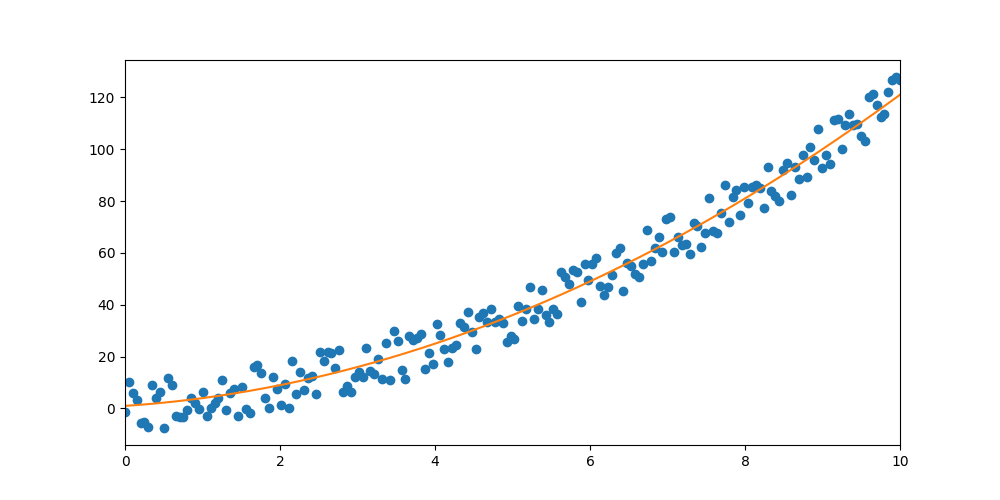
\includegraphics[width=300pt]{Regression/code/fig1.png}
\caption{Data generated from the function $f(x)=x^2+2\cdot x+1$ with added noise.}
\label{fig:linear1}
\end{figure}

In Figure \ref{fig:linear1}, the \textit{best fit} for this data is the function we used to construct it. Of course, we usually don't know the equation for the best fit beforehand, but our goal is to create a model to approximate this line as closely as possible. 

Let us start by constructing a simple machine-learning model for linear regression with no hidden layers, which essentially means there are no intermediate computations between the input and the output in our model.

Our goal is to build a machine-learning model 
$M:[0,10]\to\mathbb{R}$ of the form $$M(x) = x \cdot W + b,$$ where $W\in\mathbb{R}$ and $b\in\mathbb{R}$. Here, $W$ is called the **weight** and $b$ is called the **bias**.   

Here, we define our linear model:

\lstinputlisting[language=Python]{Regression/code/1.1.1.2.py}

In machine-learning, a model is initialized with random weights and biases, which are then corrected during training by minimizing a **loss function**. Let's start by choosing some random $W$ and $b$.

\lstinputlisting[language=Python]{Regression/code/1.1.1.3.py}
\texttt{\small{Initial weight: -0.21299332372819757 \\
Initial bias: -0.7532380921958663
}}

Given that the weight and bias was chosen at random, we don't expect it to perform very well on our data, and indeed that is the case, as shown in Figure \ref{fig:linear2}.

\begin{figure}[h]
\centering
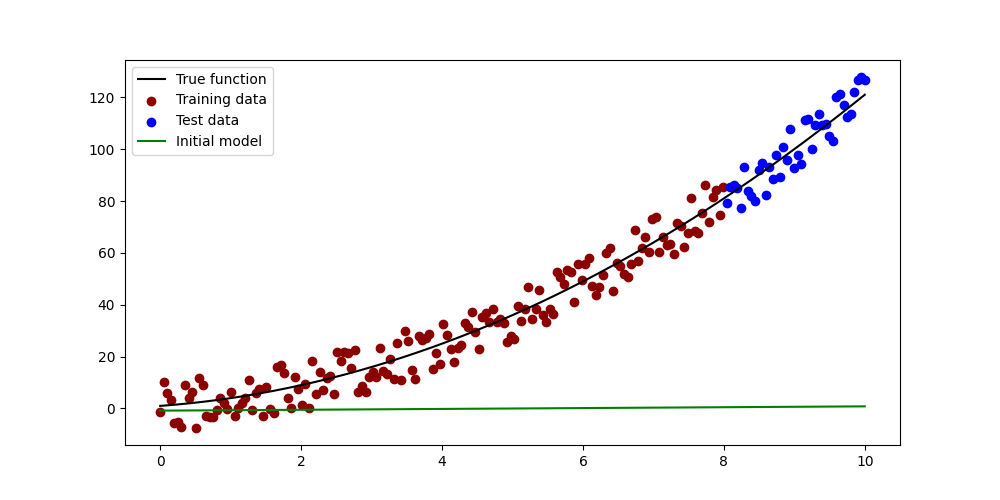
\includegraphics[width=300pt]{Regression/code/fig2.png}
\caption{Initial model prediction with random weight and bias.}
\label{fig:linear2}
\end{figure}

Let's work on improving the model. Improving our model will involve tweaking $W$ and $b$ to better fit the model using a process called \textbf{gradient descent}\index{gradient descent}.

\subsection{Gradient Descent for Univariate Linear Models}
\label{subsec:2}
We first define a \textbf{loss function}\index{loss function} to measure how our model is performing. This function will quantify the difference between the model's predictions and the actual data. A common loss function for linear regression is the \textit{Mean Squared Error} (MSE), which is defined as:
$$\mathcal{L} = MSE = \frac{1}{N}\sum_{i=1}^N\left(y_\text{i,pred} - y_\text{i,true}\right)^2.$$

\lstinputlisting[language=Python]{Regression/code/1.1.1.5.py}
\texttt{50th sample target: 21.729790078081002 \\
50th prediction: -1.2883971970405839 \\
Loss at 50th sample: 529.8369454325693 \\
Total Loss over all samples: 3485.837693509094 
}

Our goal is to minimize this loss function. 

One thing to note about this loss function is that it is a differentiable function. Recal from vector calculus that the \textbf{gradient}\index{gradient} of a differentiable funtion $f$ is a vector field $\nabla f$ whose value at point $p$ is a vector that points towards the direction of steepest ascent. 

Understanding the gradients of the loss function with respect to the model parameters—specifically, the weight $W$ and bias $b$—is crucial in machine learning, particularly when employing optimization techniques like gradient descent. Our goal is to minimize the loss function. 

The gradients $\frac{\partial \mathcal{L}}{\partial W}$ and $\frac{\partial \mathcal{L}}{\partial b}$ indicate how sensitive the loss function $\mathcal{L}$ is to changes in the parameters $W$ and $b$. In essence, they provide the direction and rate at which $\mathcal{L}$ increases or decreases as we adjust these parameters.

By computing these gradients, we can iteratively update $W$ and $b$ to minimize the loss function, thereby improving the model's performance. This process is the foundation of the gradient descent optimization algorithm.

\subsubsection{Gradients}
\begin{enumerate}
    \item \textit{Gradient with Respect to Weight $W$:}

    The partial derivative $\frac{\partial \mathcal{L}}{\partial W}$ measures how the loss changes concerning the weight $W$. A positive derivative suggests that increasing $W$ will increase the loss, while a negative derivative indicates that increasing $W$ will decrease the loss. By moving $W$ in the direction opposite to the gradient, we can reduce the loss.

    If $x_i$ is the i-th data point, let $y_{i,\text{pred}} = W \cdot x_i + b$ be the predicted value for the $i$-th data point while $y_{i,\text{true}}$ denotes the true value. Mathematically, this gradient is computed as:
    \begin{align*}
        \frac{\partial \mathcal{L}}{\partial W} &= \frac{\partial}{\partial W}\left( \frac{1}{N}\sum_{i=1}^N(y_{i,\text{pred}} - y_{i,\text{true}})^2\right) \nonumber \\
        & = \frac{1}{N}\sum_{i=1}^N\frac{\partial}{\partial W}(y_{i,\text{pred}} - y_{i,\text{true}})^2 \qquad \text{(Additive property of derivatives)} \nonumber \\
        & = \frac{1}{N}\sum_{i=1}^N\frac{\partial}{\partial W}((W\cdot x_i + b) - y_{i,\text{true}})^2 \nonumber \\
        & = \frac{1}{N}\sum_{i=1}^N 2\cdot((W\cdot x_i + b) - y_{i,\text{true}})\cdot (x_i) \qquad \text{(Chain rule)} \nonumber \\
        & = \frac{2}{N}\sum_{i=1}^N(y_{i,\text{pred}} - y_{i,\text{true}})\cdot x_i.
    \end{align*}

    Thus, we find that 
    \begin{equation}
        \frac{\partial \mathcal{L}}{\partial W} = \frac{2}{N}\sum_{i=1}^N(y_{i,\text{pred}} - y_{i,\text{true}})\cdot x_i.
        \label{eq:gradient_w}
    \end{equation}
    
    \item \textit{Gradient with Respect to Bias $ b $:}

    Similarly, the partial derivative $\frac{\partial \mathcal{L}}{\partial b}$ measures how the loss changes concerning the bias $b$. Adjusting $b$ in the direction opposite to this gradient will also help in minimizing the loss.

    This gradient is computed as:
    \begin{equation}
        \frac{\partial \mathcal{L}}{\partial b} = \frac{2}{N}\sum_{i=1}^N(y_{i,\text{pred}} - y_{i,\text{true}}).
        \label{eq:gradient_b}
    \end{equation}

    Proof of this equation is left as an exercise to the reader.
\end{enumerate}
\pagebreak
With that, we can compute the gradients in Python:

\lstinputlisting[language=Python]{Regression/code/1.1.1.6.py}

Now that we have a way of computing the partial derivatives of $\mathcal{L}$ with respect to $W$ and $b$, we can visualize the \textit{gradient field}\index{gradient field}. For a given $p=(W, b) \in \mathbb{R}^2$, the gradient $\nabla \mathcal{L}$ at $p$ is a vector that points towards the rate of fastest increase. In the following code, we compute these vectors on a grid. We also include a 2D contour plot of the loss function $\mathcal{L}$. Our initial weight $W$ and bias $b$ are marked on the plot by a red dot.

\lstinputlisting[language=Python]{Regression/code/1.1.1.7.py}

\begin{figure}
\centering
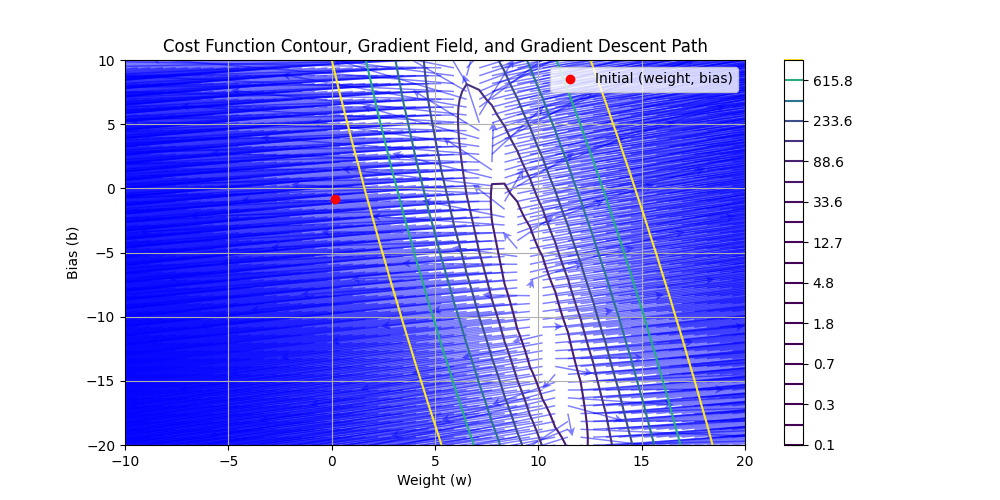
\includegraphics[width=330pt]{Regression/code/gradient-field-1.png}
\caption{Contour plot of the loss function, gradient field, and gradient descent path.}
\label{fig:linear3}
\end{figure}

Since our goal is to minimize the loss function and these vectors are pointing towards the steepest ascent of the loss function with respect to $W$ and $b$, we minimize by moving in the opposite direction of the gradients. This process is fundamental to optimization algorithms like gradient descent and is refered to as \textbf{backpropagation}\index{backpropagation} in the realm of machine-learning.

\subsubsection{Gradient Descent \& Backward Propagation}
\label{subsubsec:2}
\textbf{Gradient descent}\index{gradient descent} is an optimization algorithm that iteratively updates the model parameters in the direction opposite to the gradients of the loss function. This process continues until the loss is minimized. \textbf{Backpropagation} is the process of computing these gradients and updating the model parameters.

The parameter updates are performed iteratively using the following rules:
\begin{enumerate}
    \item  Weight update:
    $$W \leftarrow W - \alpha \frac{\partial \mathcal{L}}{\partial W}$$
   Here, $\alpha$ is the learning rate, a hyperparameter that controls the step size of each update. The term $\frac{\partial \mathcal{L}}{\partial W}$ represents the gradient of the loss function with respect to the weight. By subtracting this scaled gradient from the current weight, we move $ W $ in the direction that decreases the loss.

    \item Bias update:
    $$b \leftarrow b - \alpha \frac{\partial \mathcal{L}}{\partial b}$$
    Similarly, $\frac{\partial \mathcal{L}}{\partial b}$ is the gradient of the loss function with respect to the bias. Updating $b$ in this manner adjusts the model's predictions to better fit the data.
\end{enumerate}

The \textbf{learning rate} determines how large a step we take in the direction of the negative gradient. A small $\alpha$ leads to slow convergence, while a large $\alpha$ might cause overshooting the minimum, leading to divergence. Choosing an appropriate learning rate is crucial for effective training.

The gradients $\frac{\partial \mathcal{L}}{\partial W}$ and $\frac{\partial \mathcal{L}}{\partial b}$ indicate the direction in which the loss function increases most rapidly. By moving in the opposite direction (hence the subtraction), we aim to find the parameters that minimize the loss.

We repeat this process over and over again. Each time we do it is referred to as an \textbf{epoch}\index{epoch}. 

\lstinputlisting[language=Python]{Regression/code/1.1.1.8.py}

\texttt{\small{Initial (weight, bias): (-0.21299332372819757, -0.7532380921958663) \\
Final (weight, bias): (11.160092718469242, -10.114682847750428)
}}

\begin{figure}[H]
\centering
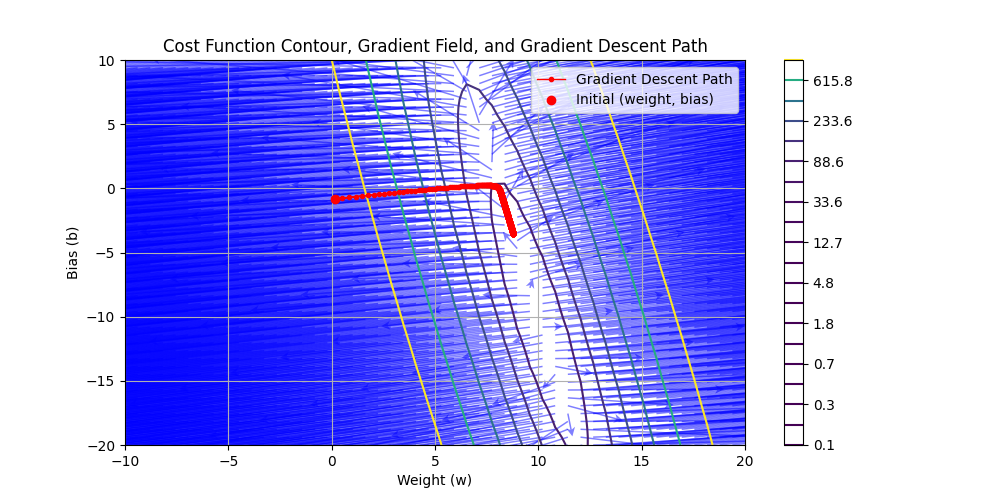
\includegraphics[width=330pt]{Regression/code/gradient-field-2.png}
\caption{Contour plot of the loss function, gradient field, and gradient descent path.}
\label{fig:linear4}
\end{figure}

Since our weight $W$ and bias $b$ together form a point $(W,b)\in\mathbb{R}^2$, the loss function $\mathcal{L}$ forms a 3-dimensional surface. The visualization below shows the path taken during gradient descent on the surface of the loss function $\mathcal{L}$. The initial point $(W,b)$ is in green. The path moves towards $\mathcal{L}$'s minimum. 

\begin{figure}[H]
\centering
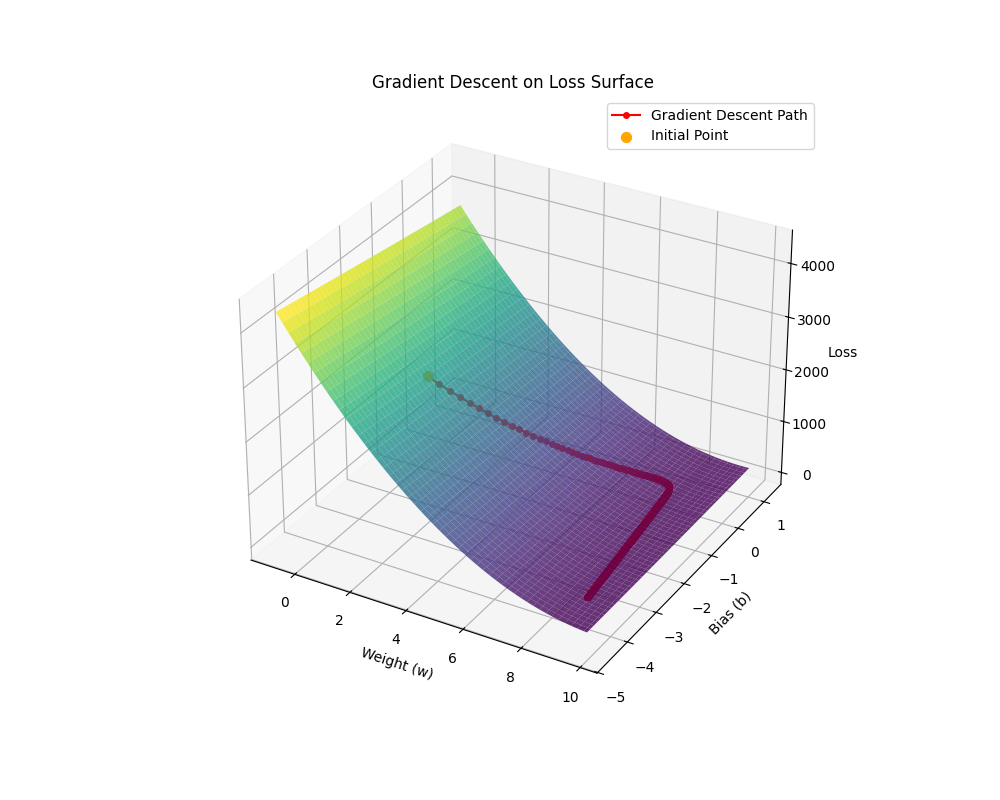
\includegraphics[width=330pt]{Regression/code/gradient-descent-3d.png}
\caption{Gradient descent path on the loss function surface. The code used to generate this visualization can be found in \ref{sec:gradient-descent-3d} of the Appendix.}
\label{fig:linear5}
\end{figure}

Finally, we visualize our initial (green) and final (red) linear model on a graph, alongside the data and true line of best fit (orange). 

\begin{figure}[H]
\centering
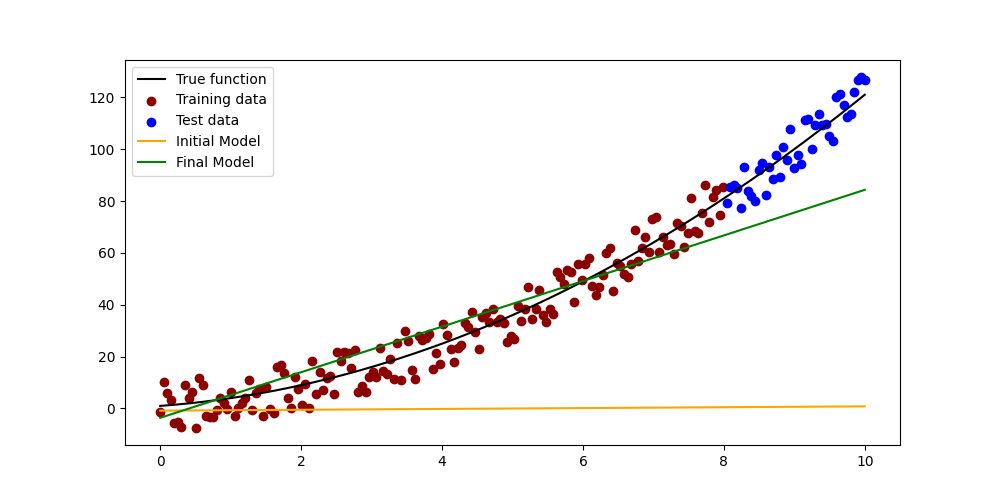
\includegraphics[width=300pt]{Regression/code/final-model.png}
\caption{Initial and final linear models compared to the true line of best fit.}
\label{fig:linear6}
\end{figure}

\subsection{Univariate Linear Models with Hidden Layers}
We build upon the ideas from the previous section by incorporating a \emph{hidden layer}\index{hidden layer} into our model, allowing it to learn intermediate representations and capture more complex patters in the data. The reason why we call it a hidden layer is because it is not directly connected to the input or output of the model. This technique involves embedding our data into higher-dimensional spaces. Higher-dimensional spaces allow for the transformation of data in a way that makes patterns, relationships, or structures more linearly separable. In lower dimensions, data that appears entangled or inseparable can often be separated in a higher-dimensional space. 

A classic example that demonstrates the concept of non-linear separability in lower dimensions but linear separability in higher dimensions is the \emph{circle classification problem}. Here, data points inside a circle belong to one class, while those outside belong to another. This problem is not linearly separable in two dimensions, but becomes linearly separable when mapped to higher-dimensional spaces using the radius as a new feature. See \ref{sec:circle-classification-visualizations} in the Appendix for the code used to generate the visualizations below.

% two figures side-by-side
\begin{figure}[H]
\centering
\begin{minipage}{.5\textwidth}
  \centering
  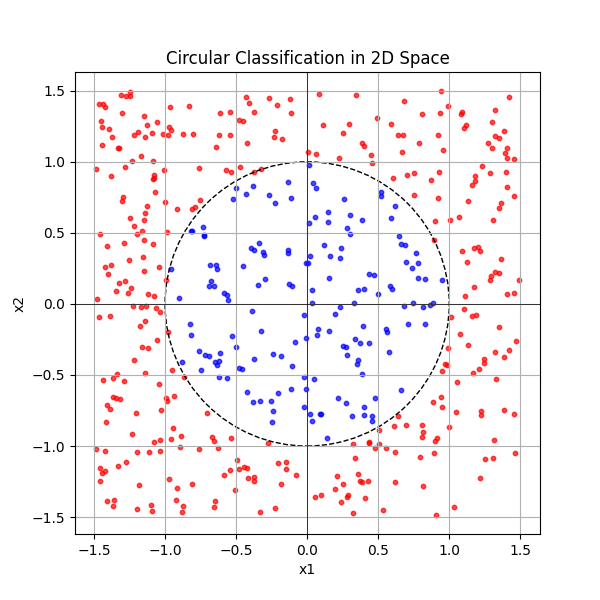
\includegraphics[width=200pt]{Regression/code/circular-data.png}
  \caption{Circle classification problem in 2D.}
  \label{fig:linear7}
\end{minipage}%
\begin{minipage}{.5\textwidth}
  \centering
  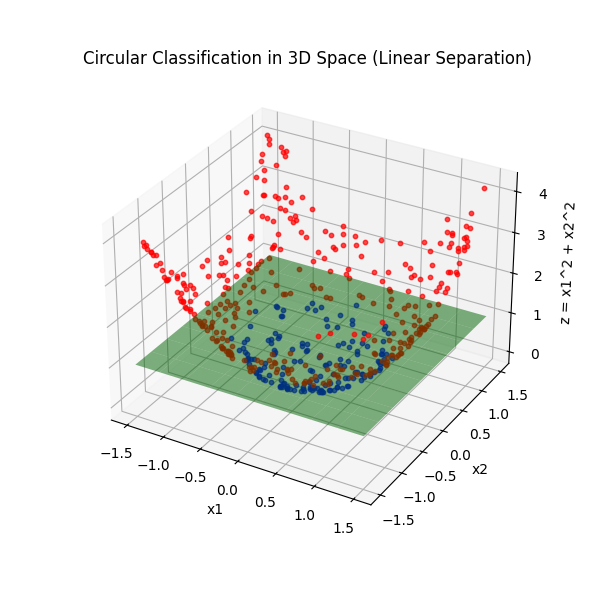
\includegraphics[width=200pt]{Regression/code/circular-data-3d.png}
  \caption{Circle classification problem in 3D.}
  \label{fig:linear8}
\end{minipage}
\end{figure}

Returning back to our linear model, let's change the model's architecture to include a hidden layer. To summarize the new model architecture:
\begin{itemize}
    \item The \textit{input layer} reshapes $x$ into a column vector $\vec{v}\in \mathbb{R}^{N\times 1}$.
    \item The \textit{hidden layer} maps $\vec{v}$ from $\mathbb{R}^{N\times 1}$ to $Z_1\in\mathbb{R}^{N\times d}$ using a linear transformation and activation function.
    \item The \textit{output layer} maps the hidden representation in $\mathbb{R}^{N\times d}$ to the final prediction $y_{\text{pred}}\in\mathbb{R}^{N\times 1}$ using a linear transformation.
\end{itemize}

\begin{enumerate}
    \item \textbf{Input Layer:}
    \begin{itemize}
        \item Takes a single real number $x\in \mathbb{R}$ as input.
        \item During training, the inputs are reshaped into a column vector $$\vec{v}=\begin{bmatrix}x_1\\x_2\\\vdots\\x_N\end{bmatrix}\in\mathbb{R}^{N\times 1},$$ where $N$ is the number of samples. We call $\vec{v}$ a \emph{batch}. Though we train with batches, inference is done on a single row at a time. 
        
        To see why training with batches still allows us to inference on a single row, see \ref{sec:training-with-batches} in the Appendix.

    \end{itemize}
    \item \textbf{Hidden Layer:}
    
    The hidden layer maps the input $\vec{v}$ from $\mathbb{R}^{N\times 1}$ to $Z_1\in\mathbb{R}^{N\times d}$, where $d$ is the hidden dimension.
    We first perform a linear transformation with the input vector:
    $$Z_1 = \vec{v}\cdot W_1 + b_1,$$
    where 
    \begin{itemize}
        \item $W_1\in\mathbb{R}^{1\times d}$ is the weight matrix,
        \item $b_1\in\mathbb{R}^{1\times d}$ is the bias vector.
        \item $Z_1\in\mathbb{R}^{N\times d}$ is the resulting representation of our vector.
    \end{itemize}
    Once the linear transformation is complete, we apply a non-linear activation function to the result. This function introduces non-linearity into the model, allowing it to learn complex patterns in the data:
    $$ A_1 = \sigma(Z_1), \quad A_1\in\mathbb{R}^{N\times d}.$$
    We will discuss activation functions in more detail soon.

    \item \textbf{Output Layer:}
    
    The hidden layer's output $A_1\in\mathbb{R}^{N\times d}$ is then passed through the output layer, which maps it to the final prediction $y_{\text{pred}}\in\mathbb{R}^{N\times 1}$ using a linear transformation:
    $$Z_2 = A_1\cdot W_2 + b_2,$$
    where
    \begin{itemize}
        \item $W_2\in\mathbb{R}^{d\times 1}$ is the weight matrix,
        \item $b_2\in\mathbb{R}^{1\times 1}$ is the bias vector,
        \item $Z_2\in\mathbb{R}^{N\times 1}$ is the intermediate prediction.
    \end{itemize}
    
    In some applications, $Z_2$ is passed through a final activation function to produce the final prediction $y_{\text{pred}}$, though for simple univariate linear regression, this step is often omitted, so 
    $$y_{\text{pred}} = Z_2.$$

\end{enumerate}

Layers are connected by an \textbf{activation function}. Activation functions should satisfy the following criteria:
\begin{itemize}
    \item \emph{Non-linearity}: The function must be non-linear to allow the model to learn complex patterns.
    \item \emph{Differentiability}: The function should be differentiable on its domain to faciliate gradient-based optimization methods like backpropagation. When we dive into models over more abstract rings, we will see how this relates to the concept of \emph{derivations} over rings.
    \item \emph{Bounded output}: Having a bounded output helps in stabilizing the learning process and prevents extreme activations.
    \item \emph{Monotonicity}: A monotonic function ensures consistent gradients, aiding in stable and efficient training.
    \item \emph{Computational efficiency}: The function should be computationally efficient to evaluate and differentiate.
\end{itemize}

A good example of such a function is the \emph{sigmoid} activation function, defined as $$\sigma(z) = \frac{1}{1 + e^{-z}}.$$ This function maps any real number to the range $(0,1)$, making it useful for many regression and classification problems. The sigmoid function is differentiable, monotonic, and computationally efficient, making it a popular choice in neural networks.

\begin{figure}[H]
\centering
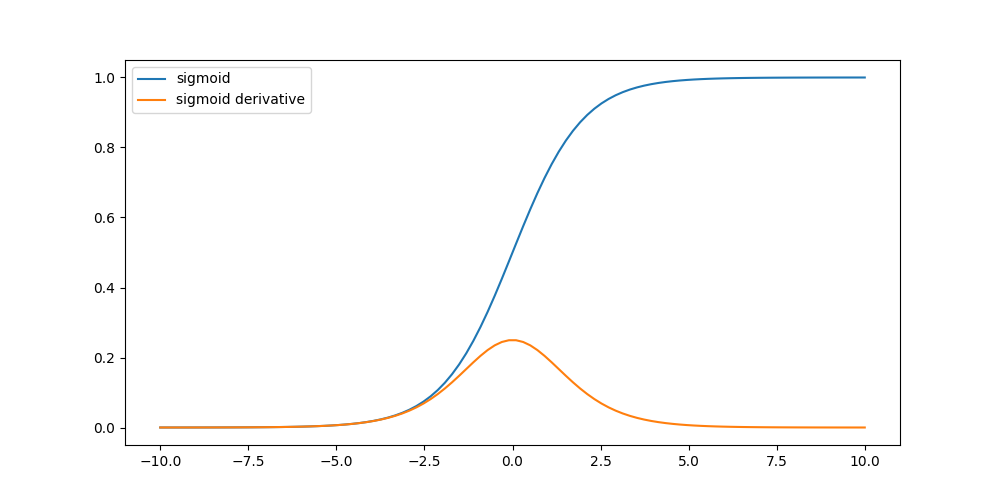
\includegraphics[width=300pt]{Regression/code/sigmoid.png}
\caption{The sigmoid activation function and its derivative.}
\label{fig:linear9}
\end{figure}

Let's implement a univariate linear model with a hidden layer with hidden dimension $d=2$ and a sigmoid activation function. We will use the same data as before.

\lstinputlisting[language=Python]{Regression/code/1.1.1.10.py}

\begin{figure}[H]
\centering
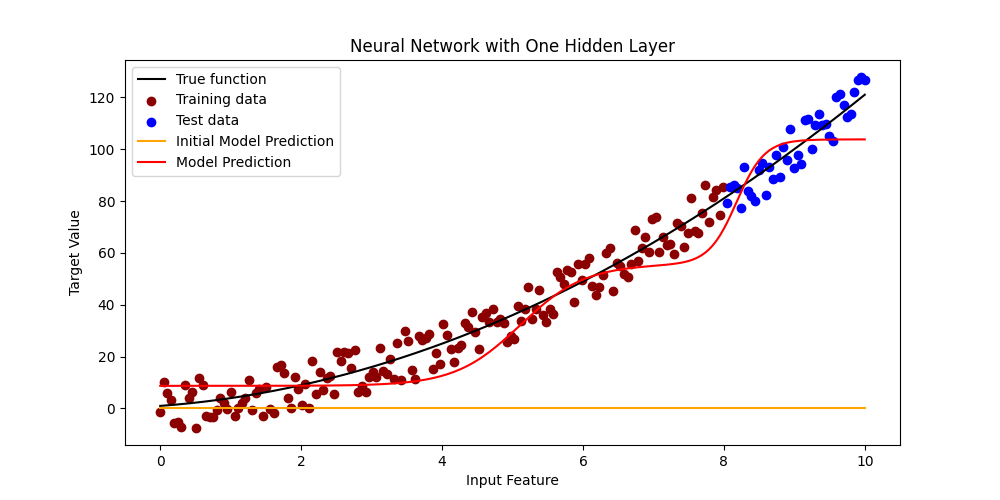
\includegraphics[width=300pt]{Regression/code/neural-network1.png}
\caption{Univariate linear model with a single hidden layer of dimension $d=2$. The initial model's state is shown, as well as its final state after training.}
\label{fig:linear10}
\end{figure}

As you can see, the model has learned that the data is not linear and has adjusted its weights and biases to better fit the data. 

Now let's train a similar model but with a hidden dimension of $d=10$.

\lstinputlisting[language=Python]{Regression/code/1.1.1.11.py}

\begin{figure}[H]
\centering
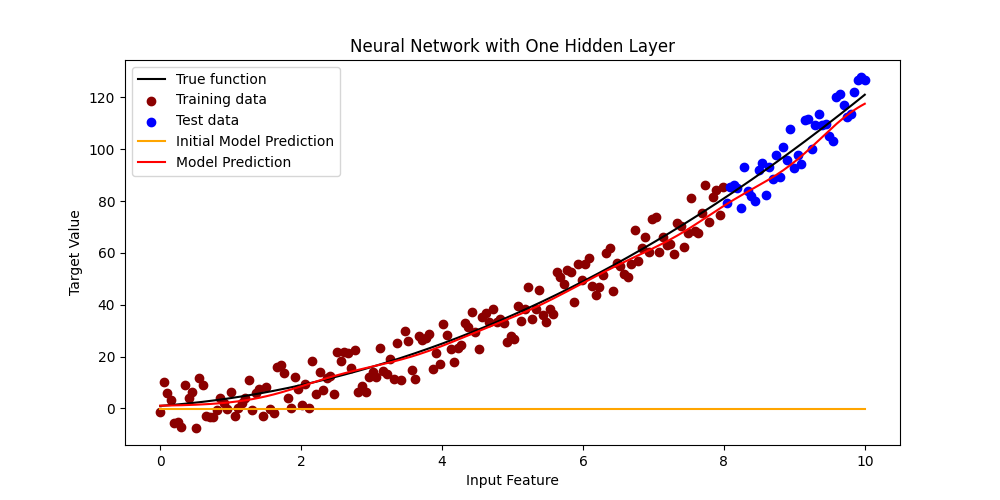
\includegraphics[width=300pt]{Regression/code/neural-network2.png}
\caption{Univariate linear model with a single hidden layer of dimension $d=10$. The initial model's state is shown, as well as its final state after training.}
\label{fig:linear11}
\end{figure}

As you can see, the higher-dimensional hidden layer allows the model to learn more complex patterns in the data and follows the true line of best fit more closely than the model with $d=2$.

%%%%%%%%%%%%%%%%%%%%%%%%% referenc.tex %%%%%%%%%%%%%%%%%%%%%%%%%%%%%%
% sample references
% %
% Use this file as a template for your own input.
%
%%%%%%%%%%%%%%%%%%%%%%%% Springer-Verlag %%%%%%%%%%%%%%%%%%%%%%%%%%
%
% BibTeX users please use
% \bibliographystyle{}
% \bibliography{}
%
\biblstarthook{In view of the parallel print and (chapter-wise) online publication of your book at \url{www.springerlink.com} it has been decided that -- as a genreral rule --  references should be sorted chapter-wise and placed at the end of the individual chapters. However, upon agreement with your contact at Springer you may list your references in a single seperate chapter at the end of your book. Deactivate the class option \texttt{sectrefs} and the \texttt{thebibliography} environment will be put out as a chapter of its own.\\\indent
References may be \textit{cited} in the text either by number (preferred) or by author/year.\footnote{Make sure that all references from the list are cited in the text. Those not cited should be moved to a separate \textit{Further Reading} section or chapter.} If the citatiion in the text is numbered, the reference list should be arranged in ascending order. If the citation in the text is author/year, the reference list should be \textit{sorted} alphabetically and if there are several works by the same author, the following order should be used:
\begin{enumerate}
\item all works by the author alone, ordered chronologically by year of publication
\item all works by the author with a coauthor, ordered alphabetically by coauthor
\item all works by the author with several coauthors, ordered chronologically by year of publication.
\end{enumerate}
The \textit{styling} of references\footnote{Always use the standard abbreviation of a journal's name according to the ISSN \textit{List of Title Word Abbreviations}, see \url{http://www.issn.org/en/node/344}} depends on the subject of your book:
\begin{itemize}
\item The \textit{two} recommended styles for references in books on \textit{mathematical, physical, statistical and computer sciences} are depicted in ~\cite{science-contrib, science-online, science-mono, science-journal, science-DOI} and ~\cite{phys-online, phys-mono, phys-journal, phys-DOI, phys-contrib}.
\item Examples of the most commonly used reference style in books on \textit{Psychology, Social Sciences} are~\cite{psysoc-mono, psysoc-online,psysoc-journal, psysoc-contrib, psysoc-DOI}.
\item Examples for references in books on \textit{Humanities, Linguistics, Philosophy} are~\cite{humlinphil-journal, humlinphil-contrib, humlinphil-mono, humlinphil-online, humlinphil-DOI}.
\item Examples of the basic Springer style used in publications on a wide range of subjects such as \textit{Computer Science, Economics, Engineering, Geosciences, Life Sciences, Medicine, Biomedicine} are ~\cite{basic-contrib, basic-online, basic-journal, basic-DOI, basic-mono}. 
\end{itemize}
}

\begin{thebibliography}{99.}%
% and use \bibitem to create references.
%
% Use the following syntax and markup for your references if 
% the subject of your book is from the field 
% "Mathematics, Physics, Statistics, Computer Science"
%
% Contribution 
\bibitem{science-contrib} Broy, M.: Software engineering --- from auxiliary to key technologies. In: Broy, M., Dener, E. (eds.) Software Pioneers, pp. 10-13. Springer, Heidelberg (2002)
%
% Online Document
\bibitem{science-online} Dod, J.: Effective substances. In: The Dictionary of Substances and Their Effects. Royal Society of Chemistry (1999) Available via DIALOG. \\
\url{http://www.rsc.org/dose/title of subordinate document. Cited 15 Jan 1999}
%
% Monograph
\bibitem{science-mono} Geddes, K.O., Czapor, S.R., Labahn, G.: Algorithms for Computer Algebra. Kluwer, Boston (1992) 
%
% Journal article
\bibitem{science-journal} Hamburger, C.: Quasimonotonicity, regularity and duality for nonlinear systems of partial differential equations. Ann. Mat. Pura. Appl. \textbf{169}, 321--354 (1995)
%
% Journal article by DOI
\bibitem{science-DOI} Slifka, M.K., Whitton, J.L.: Clinical implications of dysregulated cytokine production. J. Mol. Med. (2000) doi: 10.1007/s001090000086 
%
\bigskip

% Use the following (APS) syntax and markup for your references if 
% the subject of your book is from the field 
% "Mathematics, Physics, Statistics, Computer Science"
%
% Online Document
\bibitem{phys-online} J. Dod, in \textit{The Dictionary of Substances and Their Effects}, Royal Society of Chemistry. (Available via DIALOG, 1999), 
\url{http://www.rsc.org/dose/title of subordinate document. Cited 15 Jan 1999}
%
% Monograph
\bibitem{phys-mono} H. Ibach, H. L\"uth, \textit{Solid-State Physics}, 2nd edn. (Springer, New York, 1996), pp. 45-56 
%
% Journal article
\bibitem{phys-journal} S. Preuss, A. Demchuk Jr., M. Stuke, Appl. Phys. A \textbf{61}
%
% Journal article by DOI
\bibitem{phys-DOI} M.K. Slifka, J.L. Whitton, J. Mol. Med., doi: 10.1007/s001090000086
%
% Contribution 
\bibitem{phys-contrib} S.E. Smith, in \textit{Neuromuscular Junction}, ed. by E. Zaimis. Handbook of Experimental Pharmacology, vol 42 (Springer, Heidelberg, 1976), p. 593
%
\bigskip
%
% Use the following syntax and markup for your references if 
% the subject of your book is from the field 
% "Psychology, Social Sciences"
%
%
% Monograph
\bibitem{psysoc-mono} Calfee, R.~C., \& Valencia, R.~R. (1991). \textit{APA guide to preparing manuscripts for journal publication.} Washington, DC: American Psychological Association.
%
% Online Document
\bibitem{psysoc-online} Dod, J. (1999). Effective substances. In: The dictionary of substances and their effects. Royal Society of Chemistry. Available via DIALOG. \\
\url{http://www.rsc.org/dose/Effective substances.} Cited 15 Jan 1999.
%
% Journal article
\bibitem{psysoc-journal} Harris, M., Karper, E., Stacks, G., Hoffman, D., DeNiro, R., Cruz, P., et al. (2001). Writing labs and the Hollywood connection. \textit{J Film} Writing, 44(3), 213--245.
%
% Contribution 
\bibitem{psysoc-contrib} O'Neil, J.~M., \& Egan, J. (1992). Men's and women's gender role journeys: Metaphor for healing, transition, and transformation. In B.~R. Wainrig (Ed.), \textit{Gender issues across the life cycle} (pp. 107--123). New York: Springer.
%
% Journal article by DOI
\bibitem{psysoc-DOI}Kreger, M., Brindis, C.D., Manuel, D.M., Sassoubre, L. (2007). Lessons learned in systems change initiatives: benchmarks and indicators. \textit{American Journal of Community Psychology}, doi: 10.1007/s10464-007-9108-14.
%
%
% Use the following syntax and markup for your references if 
% the subject of your book is from the field 
% "Humanities, Linguistics, Philosophy"
%
\bigskip
%
% Journal article
\bibitem{humlinphil-journal} Alber John, Daniel C. O'Connell, and Sabine Kowal. 2002. Personal perspective in TV interviews. \textit{Pragmatics} 12:257--271
%
% Contribution 
\bibitem{humlinphil-contrib} Cameron, Deborah. 1997. Theoretical debates in feminist linguistics: Questions of sex and gender. In \textit{Gender and discourse}, ed. Ruth Wodak, 99--119. London: Sage Publications.
%
% Monograph
\bibitem{humlinphil-mono} Cameron, Deborah. 1985. \textit{Feminism and linguistic theory.} New York: St. Martin's Press.
%
% Online Document
\bibitem{humlinphil-online} Dod, Jake. 1999. Effective substances. In: The dictionary of substances and their effects. Royal Society of Chemistry. Available via DIALOG. \\
http://www.rsc.org/dose/title of subordinate document. Cited 15 Jan 1999
%
% Journal article by DOI
\bibitem{humlinphil-DOI} Suleiman, Camelia, Daniel C. O'Connell, and Sabine Kowal. 2002. `If you and I, if we, in this later day, lose that sacred fire...': Perspective in political interviews. \textit{Journal of Psycholinguistic Research}. doi: 10.1023/A:1015592129296.
%
%
%
\bigskip
%
%
% Use the following syntax and markup for your references if 
% the subject of your book is from the field 
% "Computer Science, Economics, Engineering, Geosciences, Life Sciences"
%
%
% Contribution 
\bibitem{basic-contrib} Brown B, Aaron M (2001) The politics of nature. In: Smith J (ed) The rise of modern genomics, 3rd edn. Wiley, New York 
%
% Online Document
\bibitem{basic-online} Dod J (1999) Effective Substances. In: The dictionary of substances and their effects. Royal Society of Chemistry. Available via DIALOG. \\
\url{http://www.rsc.org/dose/title of subordinate document. Cited 15 Jan 1999}
%
% Journal article by DOI
\bibitem{basic-DOI} Slifka MK, Whitton JL (2000) Clinical implications of dysregulated cytokine production. J Mol Med, doi: 10.1007/s001090000086
%
% Journal article
\bibitem{basic-journal} Smith J, Jones M Jr, Houghton L et al (1999) Future of health insurance. N Engl J Med 965:325--329
%
% Monograph
\bibitem{basic-mono} South J, Blass B (2001) The future of modern genomics. Blackwell, London 
%
\end{thebibliography}


%%%%%%%%%%%%%%%%%%%%% appendix.tex %%%%%%%%%%%%%%%%%%%%%%%%%%%%%%%%%
%
% sample appendix
%
% Use this file as a template for your own input.
%
%%%%%%%%%%%%%%%%%%%%%%%% Springer-Verlag %%%%%%%%%%%%%%%%%%%%%%%%%%

\appendix
\chapter{Python Code}
\label{introA} % Always give a unique label
% use \chaptermark{}
% to alter or adjust the chapter heading in the running headf

\section{Linear Regression}

% Always give a unique label
% and use \ref{<label>} for cross-references
% and \cite{<label>} for bibliographic references
% use \sectionmark{}
% to alter or adjust the section heading in the running head
\subsection{Code for 3D Gradient Descent Visualization}
\label{sec:gradient-descent-3d}
\begin{codeblock}
import numpy as np
import matplotlib.pyplot as plt
from mpl_toolkits.mplot3d import Axes3D

# Assuming w_history, b_history, loss_history, x, and y_data are already defined
# Create a grid of w and b values for contour plotting
w_vals = np.linspace(min(w_history) - 1, max(w_history) + 1, 100)
b_vals = np.linspace(min(b_history) - 1, max(b_history) + 1, 100)
W, B = np.meshgrid(w_vals, b_vals)

# Compute the loss for each combination of w and b in the grid
Z = np.array([mse_loss(linear_model(x, w, b), y_data) for w, b in zip(np.ravel(W), np.ravel(B))])
Z = Z.reshape(W.shape)

# Create the figure and 3D axis
fig = plt.figure(figsize=(10, 8))
ax = fig.add_subplot(111, projection='3d')

# Plot the surface
surf = ax.plot_surface(W, B, Z, cmap='viridis', alpha=0.8)

# Plot the gradient descent path
ax.plot(w_history, b_history, loss_history, color='red', marker='o', markersize=4, label='Gradient Descent Path')

# Highlight the initial point
ax.scatter(w_history[0], b_history[0], loss_history[0], color='orange', s=50, label='Initial Point')

# Add labels and a legend
ax.set_title('Gradient Descent on Loss Surface')
ax.set_xlabel('Weight (w)')
ax.set_ylabel('Bias (b)')
ax.set_zlabel('Loss')
ax.legend()

plt.savefig('gradient-descent-3d.png')
# Show the plot
plt.show()

\end{codeblock}

\subsection{Code for Circle Classification Problem Visualizations}
\label{sec:circle-classification-visualizations}
\lstinputlisting[language=Python]{Regression/code/A.1.1.2.py}

\subsection{Why Training with Batches Works}
\label{sec:training-with-batches}
During training, the input $x$ is reshaped into a column vector $\vec{v}\in\mathbb{N\times 1}$, where $N$ is the number of samples. Though our final model will process a single number $x$ during inference. The reason this works lies in how matrix operations and broadcasting work. Let's look at a simple example to gain understanding:

\begin{enumerate}
    \item \textbf{Training with a column vector:}
    
    Let's say we have three univariate data samples:
    \begin{center}
    \begin{tabular}{ |c||c|  }
        x & y \\
        \hline
        3 & -1 \\
        5 & 1 \\
        7 & 0
    \end{tabular}
    \end{center}

    Our goal is to determine the relationship between $x$ and $y$ using a linear model $y = x\cdot W +b$. Let's choose $2$ as the hidden dimension, so that $W,b\in\mathbb{R}^{1\times 2}$. We start by reshaping the input $x$ into a column vector $\vec{v}$:
    $$\vec{v} = \begin{bmatrix}
    3 \\ 5 \\ 7 
    \end{bmatrix}\in \mathbb{R}^{3\times 1}$$
    We initialize with random weight and bias:
    $$W_1 = \begin{bmatrix} 2 & -1 & \end{bmatrix} \in \mathbb{R}^{1\times 2}, \quad b_1 = \begin{bmatrix} 1 & 0 \end{bmatrix} \in \mathbb{R}^{1\times 2}.$$
    Then: 
    $$Z_1 = \vec{v}\cdot W_1 + b_1 = \begin{bmatrix} 3 \\ 5 \\ 7 \end{bmatrix} \begin{bmatrix} 2 & -1 \end{bmatrix} + \begin{bmatrix} 1 & 0 \end{bmatrix} = \begin{bmatrix} 7 & -3 \\ 11 & -5 \\ 15 & -7 \end{bmatrix}.$$

    \item \textbf{Inference with a single number:}
    
    Now that we have a model (an untrained model, but still a model), we can use it to predict the output for a new input $x=3$. We reshape $x$ into a column vector $\vec{v} = \begin{bmatrix}3\end{bmatrix} \in \mathbb{R}^{1\times 1}$ and compute the output:
    $$Z_1 = \vec{v}\cdot W_1 + b_1 = \begin{bmatrix} 3 \end{bmatrix} \begin{bmatrix} 2 & -1 \end{bmatrix} + \begin{bmatrix} 1 & 0 \end{bmatrix} = \begin{bmatrix} 7 & -3 \end{bmatrix}.$$
\end{enumerate}

\subsection{Direct Sum vs. Direct Product of Rings}
\label{sec:direct-sum-vs-direct-product}
\begin{definition}
    The \textbf{direct product} of two rings $R$ and $S$, written $R\times S$, is the Cartesian product of their elements with componentwise addition and multiplication:
    $$(r_1, s_1) + (r_2, s_2) = (r_1 + r_2, s_1 + s_2), \quad (r_1, s_1) \cdot (r_2, s_2) = (r_1 \cdot r_2, s_1 \cdot s_2).$$
    This results in a new ring $R\times S$, where $R$ and $S$ are naturally embedded as subrings:
    $$R \hookrightarrow R \times S, \quad r \mapsto (r, 0), \quad S \hookrightarrow R \times S, \quad s \mapsto (0, s).$$
    \end{definition}
    
    For finite sets, the direct product is the same as the direct sum. For infinite sets, the direct product contains **all possible tuples**, even those with infinitely many nonzero entries, which is not allowed in the direct sum.
    
    \begin{definition}
    The \textbf{direct sum} of two rings $R$ and $S$, written $R\bigoplus S$, is also the cartesian product of their elements, but with an additional restriction: in the context of abelian groups, only \textit{finitely many components are allowed to be nonzero} in the infinite case. 
    \end{definition}
    
    In the context of rings, $R\bigoplus S$ is typically defined the same as $R\times S$ for finite cases since the restriction is automatically satisfied.
    
    In machine-learning, we are mostly working with a finite number of categorical variables, so the direct sum and direct product coincide.

\backmatter%%%%%%%%%%%%%%%%%%%%%%%%%%%%%%%%%%%%%%%%%%%%%%%%%%%%%%%
%%%%%%%%%%%%%%%%%%%%%%acronym.tex%%%%%%%%%%%%%%%%%%%%%%%%%%%%%%%%%%%%%%%%%
% sample list of acronyms
%
% Use this file as a template for your own input.
%
%%%%%%%%%%%%%%%%%%%%%%%% Springer %%%%%%%%%%%%%%%%%%%%%%%%%%

\Extrachap{Glossary}

These definitions need to be redefined to make sense in the context of the book. Deciphering the jargon is a key part of understanding machine learning. Here are some common terms you might encounter:

\runinhead{Batch} A batch is a set of training examples used in one iteration of model training. The batch size is the number of examples in a batch.

\runinhead{Hidden Dimension} The hidden dimension is the number of neurons in a hidden layer of a neural network. Mathematically, it is a dimension used to construct a weight matrix and bias vector.

\runinhead{Hidden Layer} A hidden layer is a layer in a neural network that is neither an input nor an output layer. It is used to transform the input into a form that is more suitable for the output layer. Mathematically, it is a layer of neurons that applies a non-linear transformation to the input.

\runinhead{Neuron} A neuron is a single unit in a neural network that takes input, applies a transformation, and produces an output. Mathematically, it is a function that takes a weighted sum of inputs and applies an activation function. For example, a sigmoid neuron applies the sigmoid function to the weighted sum of inputs.
% 
\Extrachap{Solutions}

\section*{Problems of Chapter~\ref{intro}}

\begin{sol}{prob1}
The solution\index{problems}\index{solutions} is revealed here.
\end{sol}


\begin{sol}{prob2}
\textbf{Problem Heading}\\
(a) The solution of first part is revealed here.\\
(b) The solution of second part is revealed here.
\end{sol}


\printindex

%%%%%%%%%%%%%%%%%%%%%%%%%%%%%%%%%%%%%%%%%%%%%%%%%%%%%%%%%%%%%%%%%%%%%%

\end{document}





